% Copyright (C) 2014-2020 by Thomas Auzinger <thomas@auzinger.name>

\documentclass[draft,final]{vutinfth} % Remove option 'final' to obtain debug information.

% Load packages to allow in- and output of non-ASCII characters.
\usepackage{lmodern}        % Use an extension of the original Computer Modern font to minimize the use of bitmapped letters.
\usepackage[T1]{fontenc}    % Determines font encoding of the output. Font packages have to be included before this line.
\usepackage[utf8]{inputenc} % Determines encoding of the input. All input files have to use UTF8 encoding.

% Extended LaTeX functionality is enables by including packages with \usepackage{...}.
\usepackage{amsmath}    % Extended typesetting of mathematical expression.
\usepackage{amssymb}    % Provides a multitude of mathematical symbols.
\usepackage{mathtools}  % Further extensions of mathematical typesetting.
\usepackage{microtype}  % Small-scale typographic enhancements.
\usepackage[inline]{enumitem} % User control over the layout of lists (itemize, enumerate, description).
\usepackage{multirow}   % Allows table elements to span several rows.
\usepackage{booktabs}   % Improves the typesettings of tables.
\usepackage{caption}
\usepackage{subcaption} % Allows the use of subfigures and enables their referencing.
\usepackage[ruled,linesnumbered,algochapter]{algorithm2e} % Enables the writing of pseudo code.
\usepackage[usenames,dvipsnames,table]{xcolor} % Allows the definition and use of colors. This package has to be included before tikz.
\usepackage{nag}       % Issues warnings when best practices in writing LaTeX documents are violated.
\usepackage{todonotes} % Provides tooltip-like todo notes.
\usepackage{hyperref}  % Enables cross linking in the electronic document version. This package has to be included second to last.
\usepackage[acronym,toc]{glossaries} % Enables the generation of glossaries and lists fo acronyms. This package has to be included last.

\usepackage[draft,nomargin,inline]{fixme}
\fxsetface{inline}{\itshape}
\fxsetface{env}{\itshape}
\fxusetheme{color}

% Define convenience functions to use the author name and the thesis title in the PDF document properties.
\newcommand{\authorname}{Rupert Ettrich} % The author name without titles.
\newcommand{\thesistitle}{Using Graph Neural Networks in Local Search for Relaxations of the Maximum Clique Problem} % The title of the thesis. The English version should be used, if it exists.

% Set PDF document properties
\hypersetup{
    pdfpagelayout   = TwoPageRight,           % How the document is shown in PDF viewers (optional).
    linkbordercolor = {Melon},                % The color of the borders of boxes around crosslinks (optional).
    pdfauthor       = {\authorname},          % The author's name in the document properties (optional).
    pdftitle        = {\thesistitle},         % The document's title in the document properties (optional).
    pdfsubject      = {Subject},              % The document's subject in the document properties (optional).
    pdfkeywords     = {a, list, of, keywords} % The document's keywords in the document properties (optional).
}

\setpnumwidth{2.5em}        % Avoid overfull hboxes in the table of contents (see memoir manual).
\setsecnumdepth{subsection} % Enumerate subsections.

\nonzeroparskip             % Create space between paragraphs (optional).
\setlength{\parindent}{0pt} % Remove paragraph identation (optional).

\makeindex      % Use an optional index.
\makeglossaries % Use an optional glossary.
%\glstocfalse   % Remove the glossaries from the table of contents.

% Set persons with 4 arguments:
%  {title before name}{name}{title after name}{gender}
%  where both titles are optional (i.e., can be given as empty brackets {}).
\setauthor{}{\authorname}{BA BSc}{male}
\setadvisor{Ao.Univ.Prof. Dipl.-Ing. Dr.techn.}{Günther Raidl}{}{male}

% For bachelor and master theses:
\setfirstassistant{Projektass.}{Marc Huber}{MSc}{male}
% \setsecondassistant{Pretitle}{Forename Surname}{Posttitle}{male}
% \setthirdassistant{Pretitle}{Forename Surname}{Posttitle}{male}

% For dissertations:
% \setfirstreviewer{Pretitle}{Forename Surname}{Posttitle}{male}
% \setsecondreviewer{Pretitle}{Forename Surname}{Posttitle}{male}

% For dissertations at the PhD School and optionally for dissertations:
% \setsecondadvisor{Pretitle}{Forename Surname}{Posttitle}{male} % Comment to remove.

% Required data.
\setregnumber{01129393}
\setdate{21}{06}{2022} % Set date with 3 arguments: {day}{month}{year}.
\settitle{\thesistitle}{Using Graph Neural Networks in Local Search for Relaxations of the Maximum Clique Problem} % Sets English and German version of the title (both can be English or German). If your title contains commas, enclose it with additional curvy brackets (i.e., {{your title}}) or define it as a macro as done with \thesistitle.
% \setsubtitle{Optional Subtitle of the Thesis}{Optionaler Untertitel der Arbeit} % Sets English and German version of the subtitle (both can be English or German).

% Select the thesis type: bachelor / master / doctor / phd-school.
% Bachelor:
% \setthesis{bachelor}
%
% Master:
\setthesis{master}
\setmasterdegree{dipl.} % dipl. / rer.nat. / rer.soc.oec. / master
%
% Doctor:
%\setthesis{doctor}
%\setdoctordegree{rer.soc.oec.}% rer.nat. / techn. / rer.soc.oec.
%
% Doctor at the PhD School
%\setthesis{phd-school} % Deactivate non-English title pages (see below)

% For bachelor and master:
\setcurriculum{Logic and Computation}{Logic and Computation} % Sets the English and German name of the curriculum.

% For dissertations at the PhD School:
% \setfirstreviewerdata{Affiliation, Country}
% \setsecondreviewerdata{Affiliation, Country}

\newtheorem{theorem}{Theorem}
\newtheorem{definition}{Definition}[section]
\newtheorem{lemma}{Lemma}

\begin{document}

\frontmatter % Switches to roman numbering.
% The structure of the thesis has to conform to the guidelines at
%  https://informatics.tuwien.ac.at/study-services

\addtitlepage{naustrian} % German title page (not for dissertations at the PhD School).
\addtitlepage{english} % English title page.
\addstatementpage

\begin{danksagung*}
\todo{Ihr Text hier.}
\end{danksagung*}

\begin{acknowledgements*}
\todo{Enter your text here.}
\end{acknowledgements*}

\begin{kurzfassung}
\todo{Ihr Text hier.}
\end{kurzfassung}

\begin{abstract}
\todo{Enter your text here.}
\end{abstract}

% Select the language of the thesis, e.g., english or naustrian.
\selectlanguage{english}

% Add a table of contents (toc).
\tableofcontents % Starred version, i.e., \tableofcontents*, removes the self-entry.

% Switch to arabic numbering and start the enumeration of chapters in the table of content.
\mainmatter

\chapter{Introduction}

\section{Motivation}
In many Combinatorial Optimization Problems (COPs), problem instances exhibit clearly defined internal structures that can be expressed as graphs. Here, a graph is a tuple $G = (V, E)$, where $V$ is the set of vertices and the set of edges $E \subseteq V \times V$ defines the relationships among vertices. While there are other methods to deal with inputs of variable size (Fully Convolutional Networks, Recurrent Neural Networks), Graph Neural Networks (GNNs) are Neural Networks tailored specifically to learn from structured input in the form of graphs, making them a valuable tool for Machine Learning (ML) tasks on data with graph-like structure.   

In recent years, GNNs have gained popularity in their application in the context of COPs. However, current end-to-end ML approaches are in most cases not competitive to state-of-the-art (meta-)heuristic solution approaches, and their application is limited to small instances, where exact algorithms are available. Nonetheless, GNNs show promise in their use in COPs, and there have been many successful applications over the last years, e.g. 
% \cite{NEURIPS2021_0db2e204}, where a GNN is used to find maximal Independent Sets by imitating a time-expensive Monte-Carlo Tree Search, or
\cite{Oberweger2022}, where a Large Neighborhood Search is enhanced by a GNN that guides a destroy-operator, or \cite{NEURIPS2021_0db2e204}, where a GNN is used to find maximal Independent Sets by imitating a time-expensive Monte-Carlo Tree Search, producing solutions that reach a solution quality of $99.5\%$ while being three orders of magnitude faster. 

The main motivation of this thesis is to further study the application of GNNs in the context of metaheuristics for COPs defined on graphs. We address the problems of current end-to-end approaches by using a GNN only as a component of a metaheuristic search procedure that should enhance the search for high quality solutions either by speeding up the search or by improving the quality of its final solutions. More specifically, we consider several relaxations of a COP defined on graphs, the Maximum Clique Problem (MCP), that seem to be well-suited for our purpose. 

\section{Considered Problems}
The MCP is the problem of finding a fully connected subgraph -- a \textit{clique} -- of maximum size in a given graph. It is a fundamental problem in computer science, as its decision variant is one of Karp's 21 NP-complete problems \cite{Karp1972}. The MCP has several practical applications, e.g.,  in bioinformatics \cite{Dognin2010} and social network analysis \cite{Pattillo_network_analysis_2013}. However, for some real-world applications that require identifying dense subgraphs, the MCP is too strict a model. This leads to the introduction of several clique relaxations such as -- among others -- the Maximum Quasi-Clique Problem (MQCP) (introduced in \cite{Abello2002}, Definition \ref{def:mqcp}), the Maximum $k$-defective Clique Problem (MDCP) (introduced in \cite{Yu2006}, Definition \ref{def:mdcp}), and the Maximum $k$-plex Problem (MPP) (introduced in \cite{Seidman1978}, Definition \ref{def:mpp}). 
As all of these problems are NP-hard optimization problems, it is practically often infeasible to obtain exact solutions for large instances. However, many real-world applications often require solutions for large graphs. Therefore, efficient heuristic methods are needed that produce high quality solutions in an acceptable amount of time. While the MCP has been studied well over the last decades, heuristic methods for MQCP, MDCP, and MPP are less abundant. It is therefore another motivation of this thesis to enrich the arsenal of heuristic methods for these relaxations of the MCP. 

\section{Outline of the Thesis}

\chapter{Relaxations of the Maximum Clique Problem}

\section{Notation}

Throughout this thesis, we use standard graph theory notation. 
We consider $G = (V, E)$ to be a graph with node or vertex set $V$ and edge set $E \subseteq \{\{u,v\} \mid u,v \in V\}$. We use the terms node, nodes and vertex, vertices interchangeably when denoting elements of $V$. 
A graph $G$ is \emph{simple}, if it contains no self-loops (e.g.,  $\{v,v\} \in E$) or multiple edges between two vertices. In this thesis, we only consider unweighted, undirected, simple graphs, as all the considered problems are defined on such graphs. 
A graph $G' = (V', E')$ is a subgraph of $G = (V,E)$ iff $V' \subseteq V$, $E' \subseteq E$, and $\{u,v\} \in E' \colon u,v \in V'$. Let $S \subseteq V$ be a set of vertices in $G$. The subgraph induced by $S$ in $G$, denoted as $G[S]$, is a graph with vertex set $S$ and edge set $E(S) = \{ \{u,v\} \mid \{u,v\} \in E, u,v \in S \}$. 
A \emph{clique} is a set of vertices $S \subseteq V$ such that $G[S]$ is fully connected, i.e., $|E(S)| = \frac{|S| \cdot (|S|-1)}{2}$. A fully connected graph on $n$ nodes is denoted as $K_n$.
The density $dens(G)$ of a graph $G = (V,E)$ is defined as the ratio of the number of edges $|E|$ to the number of edges in a fully-connected graph with $|V|$ nodes $\binom{|V|}{2}$. The density of a graph is therefore a rational number between zero and one. 


\section{The Maximum Clique Problem}

The Maximum Clique Problem (MCP, Definition \ref{def:mcp}) is a fundamental problem in graph theory and computer science. Its decision variant was one of first problems that were shown to be NP-Complete \cite{Karp1972}, from which NP-hardness can be derived for the maximization variant. The MCP is a well-studied problem and has many real-world applications, e.g.,  in social network analysis, bioinformatics, and telecommunication \todo{include citations}. 
Figure \ref{fig:maxclique} depicts a maximum clique in a graph. 
\begin{figure}
    \centering
    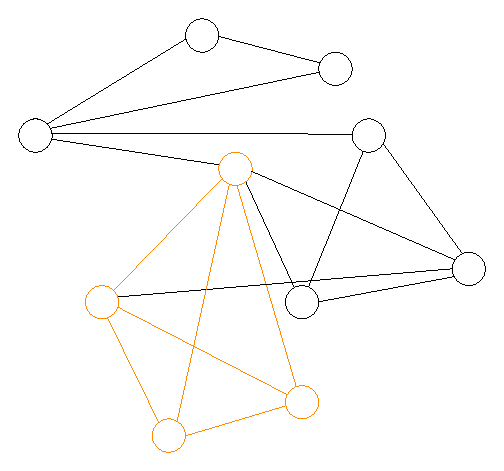
\includegraphics[width=0.3\textwidth]{graphics/graph1-clique.eps}
    \caption{A maximum clique.}
    \label{fig:maxclique}
\end{figure}
For some real-world applications however, the MCP is too strict a model, as some applications require identifying large, dense subgraphs, but not necessarily fully connected subgraphs. This leads to the introduction of several relaxations of the maximum clique problem. \todo{list relevant relaxations}

\begin{definition}[Maximum Clique Problem]
	\label{def:mcp}
	Given a graph $G = (V,E)$, the Maximum Clique Problem (MCP) is the problem of finding clique of maximum size in $G$. 
\end{definition}

\subsection{Properties of the MCP}
\todo{not approximable}

\section{The Maximum Quasi-Clique Problem}

\begin{definition}[Maximum Quasi-Clique Problem]
	\label{def:mqcp}
	Given a graph $G = (V,E)$ and $\gamma \in (0,1]$, the Maximum $\gamma$-Quasi-Clique Problem (MQCP) is the problem of finding a subset of vertices $S \subseteq V$ of maximum size 
	such that the induced subgraph $G[S]$ has an edge density of at least $\gamma$, or, in other words, $G[S]$ contains at least $\gamma \binom{|S|}{2}$ edges. 
\end{definition}

\subsection{Properties of the MQCP}


\subsection{Preprocessing of MQCP Instances}

In \cite{Abello2002}, the authors introduce the notion of $\gamma k$\emph{-peelable} vertices in the context of preprocessing. A vertex $v$ is $\gamma k$\emph{-peelable} if $v$ and all its neighbors have degree smaller than $\gamma k$. If a lower bound $k$ for the size of a maximum $\gamma$-quasi clique is known, the authors propose to remove all edges incident to $\gamma k$\emph{-peelable} vertices from $G$ in preprocessing. This preprocessing rule might be used to speed up the search process by sparsifying the graph, but we note that this preprocessing rule does not necessarily preserve the existence of optimal solutions. We prove this claim by giving a counterexample in Figure \ref{fig:preprocessing-mqcp-counterexample}, where the optimal solution cannot be obtained after applying said preprocessing rule. 


\begin{figure}
    \centering
    \begin{subfigure}{.5\textwidth}
      \centering
      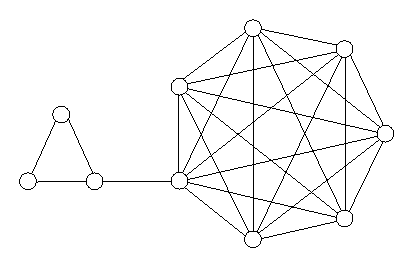
\includegraphics[width=.9\linewidth]{graphics/preprocessing-mqcp-counterexample-1.eps}
      \caption{The original graph instance.}
      \label{fig:preprocessing-mqcp-sub1}
    \end{subfigure}%
    \begin{subfigure}{.5\textwidth}
      \centering
      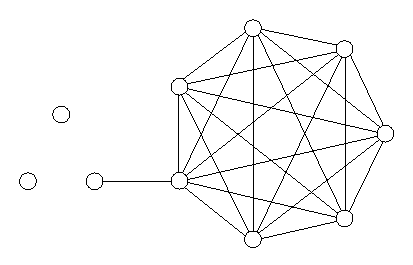
\includegraphics[width=.9\linewidth]{graphics/preprocessing-mqcp-counterexample-2.eps}
      \caption{The graph instance after preprocessing.}
      \label{fig:preprocessing-mqcp-sub2}
    \end{subfigure}
    \caption{Consider the graph $G$ given in Subfigure \ref{fig:preprocessing-mqcp-sub1}. The considered MQCP instance is defined by $G$ consisting of a $K_3$ and a $K_7$ connected by an edge and $\gamma=0.5$. Since $G$ has a density $dens(G) = \frac{25}{45} \approx 0.56$, the maximum $0.5$-quasi clique in $G$ is $V$. Assume a lower bound of $k=6$ is known, therefore the two nodes on the left are $k\gamma$\emph{-peelable} and preprocessing would remove all edges incident to these vertices, as can be seen in Subfigure \ref{fig:preprocessing-mqcp-sub2}. Therefore, the density of this preprocessed graph would be reduced to $\frac{22}{45} \approx 0.49$ and the optimal solution $V$ would not be preserved.}
    \label{fig:preprocessing-mqcp-counterexample}
\end{figure}


\section{The Maximum k-defective Clique Problem}

\begin{definition}[Maximum $k$-defective-Clique Problem]
	\label{def:mdcp}
	Given a graph \\ 
    $G = (V,E)$ and integer $k$, the Maximum $k$-defective Clique Problem (MDCP) is the problem of finding a subset of vertices $S \subseteq V$ of maximum size 
	such that the induced subgraph $G[S]$ contains at least $\binom{|S|}{2} - k$ edges. 
\end{definition}

\section{The Maximum k-plex Problem}

\begin{definition}[Maximum $k$-plex Problem]
	\label{def:mpp}
	Given a graph $G = (V,E)$ and integer $k$, the Maximum $k$-plex Problem (MPP) is the problem of finding a subset of vertices $S \subseteq V$ of maximum size 
	such that each $v \in S$ is adjacent to at least $|S| - k$ vertices in $S$. 
\end{definition}

\chapter{Related Work}

\section{Machine Learning in Combinatorial Optimization Problems}

\section{Graph Neural Networks in Combinatorial Optimization Problems}

\section{Solution Approaches for the MQCP}
\subsection{Exact Approaches}\label{milp-mqcp}
Pattillo et al. \cite{pattillo_maximum_2013} propose a Mixed Integer Linear Programming formulation with a number of variables that is quadratic in the size of the vertex set $V$. 
It is derived from the following quadratic formulation, where $x_i \in \{0,1\}$ are binary decision variables representing the solution set $S \subseteq V$, and $a_{ij}$ represent elements of the adjacency matrix with $a_{ij}$ equal to one if $\{i,j\} \in E$ and zero otherwise: 

\fxnote{GR: MILPs schreibt man normalerweise so auf, dass die Zielfunktion und alle Funktionen linksbündig stehen, alle Quantoren rechtsbündig. Inequalities nicht in eine Zeile zusammenfassen (außer Domainangaben wie 0 <= x <= 10.)}
\begin{align}
    \max \sum_{i=1}^{n} x_i & \\
    \text{s.t. } \sum_{i=1}^n \sum_{j=i+1}^n a_{ij} x_i x_j & \geq \gamma \sum_{i=1}^n \sum_{j=i+1}^n x_i x_j
\end{align}
The authors linearize the above quadratic formulation by introducing variables $w_{ij}$ defined as $w_{ij} = x_i x_j$: 

\begin{align}
    \max & \sum_{i=1}^n x_i \\
    \text{s.t. } & \sum_{i=1}^n \sum_{j=i+1}^n (\gamma - a_{ij}) w_{ij} \leq 0  
\end{align}
\begin{align}
    w_{ij} &\leq x_i, & & w_{ij} \leq x_j, & & w_{ij} \geq x_i + x_j - 1, & & j > i=1, \dots , n \\
    w_{ij} &\geq 0,   & & x_i \in \{0,1\}, & & j > i = 1, \dots, n        & & 
\end{align}

\subsection{Heuristic Approaches}

\subsubsection{Construction Heuristics}

\subsubsection{Population Based Heuristics}

\subsubsection{Local Search Based Metaheuristics}

\chapter{Methodology}

\section{Machine Learning}

\subsection{Neural Networks}

\subsection{Graph Neural Networks}

\section{Local Search}

\subsection{Tabu Search}

\section{Beam Search}

\section{Linear Programming}


\chapter{Local Search with Graph Neural Networks}

\fxnote{GR: Wie glaube ich schon kurz besprochen würde ich das ganze Verfahren nicht als Local Search bezeichnen, mit den ganzen enthaltenen Techniken ist es schon ``mehr'', d.h. eine Metaheuristik, evtl. eine Tabusuche etc.? Jedenfalls sollte man sich aber auch möglichst an die Literatur in den Bezeichnungen anlehnen. Das gilt dann auch für den Gesamttitel der Arbeit. }
In this chapter we present the main contribution of this thesis in detail: a local search algorithm using Graph Neural Networks. 
At first, we introduce the general structure of the algorithm without using GNNs in Section \ref{sec:algorithm-structure}. We present two types of construction heuristics that we use in our algorithm. The first one is used to efficiently obtain a feasible initial solution of high quality that can be used as a lower bound, whereas the second one does not necessarily yield a feasible solution, but is used to explore new regions of the search space not yet visited. In Section \ref{sec:neighborhood-structure} we define the main move operator used in the local search procedure and define the corresponding neighborhood structures. Furthermore, we show in detail the local search procedure of our algorithm that utilizes said neighborhood structures. Section \ref{sec:gnn-local-search} presents our idea of utilizing a GNN to the previously described local search algorithm. In Section \ref{sec:gnn-training} we show how training data is generated and how target values are obtained. Finally, our proposed GNN architecture is presented in \ref{sec:gnn-architecture}.

\section{Algorithm Structure} \label{sec:algorithm-structure}

\fxnote{GR: Referenzen, auf welche Arbeit(en) der Algorithmus aufbaut!}
The pseudocode of the general structure of the local search algorithm is shown in Algorithm \ref{alg:structure}.
$InitialSolution$ constructs a feasible initial solution. Its main purpose is to obtain a high quality lower bound to obtain a good starting value for $k$. The procedure is described in detail in Section \ref{sec:construction-heuristics}.
\fxnote{GR: $Freq$ ist generll als $\mathit{Freq}$ zu schreiben, gilt auch für ConstructionHeuristic, Extended etc.} In line \ref{alg:structure-freq} a long-term memory $Freq$ is initialized, where $Freq[i]$ stores how many times each node is operated on for $i=1,\dots,n$. This memory is kept when the loop in lines \ref{alg:structure-while-start}--\ref{alg:structure-while-end} is repeated, but no feasible solution could be found. In $ConstructionHeuristic$, $Freq$ is used to produce a candidate solution that favors nodes that have not been considered yet. This way, new regions of the search space are explored. The candidate solution obtained in line \ref{alg:structure-construction} is then improved by the local search procedure, which is described in detail in Section \ref{sec:neighborhood-structure} along with the definition of the neighborhood structures. If the resulting solution $S$ is feasible, a simple search is performed in $Extend$ to check if the solution can be extended to a feasible solution of greater size as shown in Algorithm \ref{alg:extend}.
Furthermore, $k$ is increased, $Freq$ is reset, and the best-so-far found solution $S^*$ is updated. 
If the solution obtained by the local search procedure is not feasible, the while-loop is repeated until the stopping criterion is met, e.g.,  the time limit is reached. 

\begin{algorithm}
    \DontPrintSemicolon
    \KwIn{Graph $G$, Target Density $\gamma$}
    \KwOut{Approximate maximum $\gamma$-quasi clique in $G$}
    $S^* \gets InitialSolution(G, \gamma)$ \;
    $k \gets |S^*|$ \;
    $Freq \gets [0, \dots, 0]$ \label{alg:structure-freq} \tcp*{$n$-element Array, initialized with 0} 

    \While{stop condition not met}{ \label{alg:structure-while-start}
        $S \gets ConstructionHeuristic(G, Freq, k)$ \; \label{alg:structure-construction}
        $S \gets LocalSearch(G, Freq, \gamma, S)$ \;
        \If{$S$ is feasible}{
            $S \gets Extend(G, S, \gamma)$ \;
            $S^* \gets S$ \;
            $k \gets |S| + 1$ \;
            $Freq \gets [0, \dots, 0]$ \; 
        }\label{alg:structure-while-end}
    }
    \Return{$S^*$}
    \caption{Structure of the Local Search Algorithm}
    \label{alg:structure}
\end{algorithm}

\begin{algorithm}
    \DontPrintSemicolon
    \KwIn{Graph $G$, Feasible solution $S$, Target Density $\gamma$}
    \KwOut{Feasible solution $S^\prime$ of size at least $|S|$}
    $S^\prime \gets S$ \;
    \While{$true$}{\label{alg:extend-while-start}
        \For{$u \in V \setminus S^\prime$}{
            \If{$S^\prime \cup \{u\}$ is a $\gamma$-Quasi Clique}{
                $S^\prime \gets S^\prime \cup \{u\}$ \;
                \textbf{continue} while-loop in line \ref{alg:extend-while-start} \;
            }
        }
        \textbf{break} out of while-loop
    }
    \Return{$S^\prime$}
    \caption{Extend a feasible solution}
    \label{alg:extend}
\end{algorithm}

\section{Construction Heuristics}\label{sec:construction-heuristics}

\fxnote{GR: Ein Beam Search ist keine Konstruktionsheuristik! Bitte diese Begriffe wirklich trennen.}

\fxnote{GR: Auch hier sollten ggfs.\ aus der Literatur übernommene Ideen/Konzepte mit entsprechenden Referenzen belegt werden.}
We propose two different construction heuristics. The first one is based on Beam Search and returns a feasible solution that can be used as a lower bound for the size of a maximum $\gamma$-quasi clique in the input graph. The pseudocode is shown in Algorithm~\ref{alg:initial-construction}. We use a simple data structure for nodes of the beam search tree with fields $node.S$ containing a feasible $\gamma$-quasi clique that this node represents, and $node.g$, which is the value of the node according to the used guidance function. The root node of the beam search tree is defined by an empty candidate set and $node.g=0$. The main loop in line \ref{alg:exploration-construction-while-start}-\ref{alg:exploration-construction-while-end} expands all nodes in the current beam into all feasible successor nodes. Since a node represents a feasible $\gamma$-quasi clique, successor nodes are generated by checking for all $u \in V \setminus node.S$ whether $node.S \cup \{u\}$ is still a feasible $\gamma$-quasi clique. These successor nodes are then added to a list $children$. All nodes in $children$ are evaluated by a guidance function $g$, and the $\beta$ nodes with highest $g$-values form a new beam while the remaining nodes are discarded. 
\fxnote{GR: Die Guidance Function entspricht ja nicht dem $g$-Wert der Knoten, daher sollte diese anders benannt werden. Üblich ist $f(u)=g(u)+h(u)$, wo $g(u)=node.g$ der Value von $u$ ist und $h(u)$ der value-to-go, d.h., i.A. ein geschätzter Wert um wieviel der aktuelle Wert im besten Fall noch gesteigert werden kann.}
Since all the solutions corresponding to nodes on a level of the search tree have the same cardinality, a random node is selected to possibly update the best-so-far solution $S^*$ on each level.
Finally, the maximum cardinality solution is returned. 

We propose two different guidance functions for this beam search construction heuristic: 
\begin{itemize}
    \item The first one returns the solution size that is obtained by a simple greedy construction: Given a node with candidate set $S$, greedily add the node $v = \arg \max_{u \in V \setminus S} d_S(u)$ if $S \cup \{v\}$ is still a feasible $\gamma$-quasi clique, where $d_S(u) = |\{v \mid v \in S, \{u,v\} \in E \}|$. Ties are broken randomly. The size of the solution obtained this way is then the return value of the guidance function. This guidance function has a time complexity of $O(kn)$ per iteration, where $k$ is the solution size obtained by the greedy construction and $n$ is the number of nodes in $G$. 
    \item The second guidance function evaluates a node with candidate set $S$ by calculating the sum of the $d$ nodes in $V \setminus S$ with the highest values for $d_S(u)$. \fxnote{GR: Was ist $d$? Hier gibt es auch einen Nameclash mit $d_s$.} This guidance function is designed to be more time-efficient than the previous one. 
\end{itemize}


\begin{algorithm}
    \DontPrintSemicolon
    \KwIn{Graph $G$, Target density $\gamma$, guidance function $g$, beam width $\beta$}
    \KwOut{A feasible $\gamma$-quasi clique $S$}
    $root.S \gets \emptyset$ \;
    $S^* \gets \emptyset$ \;
    $beam \gets \{root\}$ \;
    \While{$beam$ not empty}{\label{alg:initial-construction-while-start}
        $children \gets \emptyset$ \;
        \For{$node \in beam$}{
            Expand $node.S$ into all feasible solutions that can be obtained by adding a node from $V \setminus node.S$ \;
            $children \gets $ add feasible solutions obtained from $node$ \;
        }
        \If{$children$ not empty}{
            $S^* \gets node.S$ for some arbitrary node in $children$ 
        }
        Evaluate nodes in $children$ by guidance function $g$ \;
        $beam \gets $ Choose $\beta$ nodes with highest $g$-values
    }\label{alg:initial-construction-while-end}
    \Return{$S^*$}
    \caption{Construction Heuristic based on Beam Search}
    \label{alg:initial-construction}
\end{algorithm}

The second construction heuristic has a different goal: It aims to return a set of nodes $S$ of fixed size $|S| = k$ that is promising to lead to new local optima when used as a starting point for the local search procedure. The candidate solution returned by this construction heuristic is not necessarily feasible. 
It is based on a GRASP-like randomized construction, but includes a parameter $p \in \{0,1\}$ which controls the balance between choosing nodes that have not been explored yet and nodes that increase the objective value of the current candidate solution. This approach of balancing exploration and objective value is inspired by \cite{chen_nuqclq_2021}, where the authors use a similar strategy during construction. We combine this idea with using a GRASP-like approach. The procedure is shown in Algorithm \ref{alg:exploration-construction}. At first, a starting node is selected by choosing a node with the lowest $Freq$-value, breaking ties randomly. In each iteration of the main while loop in line \ref{alg:exploration-construction-while-start}-\ref{alg:exploration-construction-while-end}, with probability $p$ a node with the lowest $Freq$-value in $N_G(S)$ is added to the current candidate solution $S$. If $N_G(S)$ is empty, an arbitrary node with the lowest $Freq$ value from $V\setminus S$ is selected instead. 
\fxnote{GR: Was ist $N_G$(S)? Ist nicht definiert.}
With probability $1-p$ we perform an iteration of a GRASP-like randomized construction: The restricted candidate list $RCL$ is built by adding all nodes from $V \setminus S$ that fulfill the condition $d_S(u) \geq d_{\max} - \alpha(d_{\max} - d_{\min})$, where $d_S(u)$ denotes the number of neighbors in $S$ for a node $u \in V \setminus S$, and $d_{\max}, d_{\min}$ are the maximum and minimum values $d_S(u)$ over all nodes $u\in V \setminus S$. Here, the parameter $\alpha$ controls the balance between greediness and randomness in a GRASP-like manner: $\alpha=0$ corresponds to a greedy strategy, whereas $\alpha=1$ corresponds to a purely random strategy.  

\begin{algorithm}
    \DontPrintSemicolon
    \KwIn{Graph $G$, $n$-element array $Freq$, Target size $k$, GRASP parameter $\alpha$, Exploration parameter $p$}
    \KwOut{Candidate set $S$}
    $u \gets $ node in $G$ with lowest $Freq$-value, break ties randomly \;
    $S \gets \{u\}$ \;
    \While{$|S| < k$}{\label{alg:exploration-construction-while-start}
        \uIf{$rand() < p$}{
            \uIf{$N_G(S)$ not empty}{
                $u \gets$ Pick random neighbor in $N_G(S)$ with lowest $Freq$-value\;
            }
            \Else{
                $u \gets$ Pick random node in $V \setminus S$ with lowest $Freq$-value
            }
        }
        \Else{
            $d_{\min} = \min_{u \in V \setminus S} d_S(u)$ \;
            $d_{\max} = \max_{u \in V \setminus S} d_S(u)$ \;
            $RCL \gets \{ u \mid u \in V\setminus S, d_S(u) \geq d_{\max} - \alpha(d_{\max} - d_{\min}) \}$ \;
            $u \gets $ Pick random node from $RCL$ \;
        }
        $S \gets S \cup \{u\}$ \;
    }\label{alg:exploration-construction-while-end}
    \Return{$S$}
    \caption{Construction Heuristic with focus on exploration}
    \label{alg:exploration-construction}
\end{algorithm}

\section{Neighborhood Structure and Local Search} \label{sec:neighborhood-structure}

The neighborhood of a candidate solution $S$ is defined by a move operator that swaps a node $u \in S$ with a node $v \in V \setminus S$. The set of neighboring candidate solutions of $S$ with $|S| = k$ that can be obtained by a single swap move is therefore defined as $\Omega_1 = \{ S \setminus \{u\} \cup \{v\} \mid u \in S, v \in V \setminus S \}$ and has size $|\Omega_1| = k \cdot (|V|-k)$, which is in $O(|V|^2)$. Similarly, we define $\Omega_d$ for $d=1,2,3,\dots$ as the set of neighboring solutions that can be obtained by swapping $d$ nodes from $S$ with $d$ nodes from $V \setminus S$, obtaining a neighborhood of size $|\Omega_d| = \binom{k}{d} \cdot \binom{|V|-k}{d}$, which is in $O(|V|^{2d})$. 


The quality of a candidate solution depends on the considered problem. For the MQCP and the MDCP a candidate solution $S$ is of higher quality than a neighboring solution $S^\prime$ if $G[S]$ contains more edges than $G[S']$. Thus, we define the objective function $f \colon 2^V \rightarrow \mathbb{N}$ for the local search for MQCP and MDCP as the function that maps a subset of vertices $S \subseteq V$ to the number of edges in the induced subgraph $G[S]$. Therefore, $S$ is better than $S^\prime$ if and only if $f(S) > f(S^\prime)$. 

Similar algorithms that use local search in order to improve a candidate solution (e.g.,  \cite{chen_nuqclq_2021}, \cite{djeddi_extension_2019}, \cite{zhou_opposition-based_2020}) only search the neighborhood $\Omega_1$ for improving solutions. As the size of this neighborhood is already quadratic in $|V|$, the authors of the mentioned algorithms restrict the neighborhood to promising moves. A scoring function is used to find promising nodes in $V \setminus S$ and in $S$ that can be used for swaps. This scoring function is in most cases defined as $d_S(u) = |\{v \mid v \in S, \{u,v\} \in E \}|$. This way, the change in the objective function value when swapping a node $u \in S$ with a node $v \in V \setminus S$ can efficiently be calculated by $\Delta_{uv} = d_S(v) - d_S(u) - e_{uv}$, where $e_{uv} = 1$ if $\{u,v\} \in E$ and $e_{uv} = 0$ otherwise. 
The scoring function $d_S$ is thus used to restrict the neighborhood $\Omega_1$. 
Let $d_{\min} = \min_{u \in S} d_S(u)$ and $d_{\max} = \max_{u \in V \setminus S} d_S(u)$.
\fxnote{GR: Diese Definitionen stehen etwas formloser oben schon, besser nur einmal sauber oben definieren.} Furthermore, let $X = \{ u \mid u \in S, d_S(u) \leq d_{\min} + 1 \}$ and $Y = \{ v \mid v \in V \setminus S, d_S(v) \geq d_{\max} - 1 \}$. The neighborhood $\Omega_1$ of a candidate solution $S$ is then restricted to only those neighboring solutions that can be obtained by swapping a node $u \in X$ with a node $v \in Y$, as all node swaps that maximize $\Delta_{uv}$ are contained in this restricted neighborhood. 

The pseudocode for our local search procedure is shown in Algorithm \ref{alg:local-search-procedure}. 
In each iteration of the main while-loop the restricted candidate sets $X$ and $Y$ are created from the sets $S$ and $V \setminus S$, respectively. These sets are created as described before, with an additional restriction: To prevent cycling through the same candidate solutions over and over again, a short-term memory is used to further restrict the sets $X$ and $Y$. There are two main methods that can be found in the literature, which we want to evaluate in our algorithm: 
\begin{itemize}
    \item In \cite{djeddi_extension_2019} and \cite{zhou_opposition-based_2020}, a tabu list is used to prevent cycling. Each time a vertex is in or out of the solution, it is added to the tabu list for a fixed number of iterations. While a vertex is in the tabu list, it is blocked and cannot be used in swaps. In \cite{djeddi_extension_2019}, the authors use two tabu lists: One for moving vertices out of the candidate solution, and one for adding vertices to the candidate solution. In \cite{zhou_opposition-based_2020}, a single tabu list is used for both operations. 
    \item In \cite{chen_nuqclq_2021}, the authors use Configuration Checking. In its simplest form, once a vertex $v$ is moved out of the candidate Solution, it is blocked from being moved again until at least one neighbor of $v$ is moved. The authors refine this strategy by using a threshold for each node $v$ that starts with $threshold(v) = 1$ for all $v \in V$. Each time a vertex $v$ is moved into the candidate solution, $threshold(v)$ is increased by 1. When $v$ is moved out of the candidate solution, it is blocked from being moved again, until $threshold(v)$ of its neighbors have been moved. Additionally, if $threshold(v) > ub\_threshold$, where $ub\_threshold$ is a user-defined upper bound, then $threshold(v)$ is reset to 1. 
\end{itemize}
If no improving move is possible, or one of the sets $X, Y$ is empty, a swap of two randomly selected unblocked vertices is performed in order to diversify the current local optimum. Furthermore, we define as stopping criteria: If the best solution $S^*$ does not improve for a fixed amount of iterations $it$, the procedure is stopped and $S^*$ is returned. Additionally, if a given time limit is reached, the procedure is stopped as well. 

\begin{algorithm}
    \DontPrintSemicolon
    \KwIn{Graph $G$, Frequency list $Freq$, Target density $\gamma$, Candidate solution $S$}
    \KwOut{Best found solution $S^*$}
    $k \gets |S|$ \;
    $S^* \gets S$
    \While{stop criterion not met}{
        $X \gets $ restricted candidate set from $S$ \;
        $Y \gets $ restricted candidate set from $V \setminus S$ \;
        \uIf{$X$ or $Y$ empty}{
            Choose arbitrary unblocked $u \in S, v \in V \setminus S$\;
        }
        \uElseIf{there exists $u \in X, v \in Y$ with positive $\Delta{uv}$}{
            $u,v \gets $ Choose $u \in X, v \in Y$ with positive $\Delta{uv}$ \;
        }
        \Else{
            \tcp{No improving move possible}
            $u,v \gets $ Choose $u \in X, v \in Y$ arbitrarily
        }
        $S \gets $ solution obtained by swapping $u \in X, v \in Y$ \;
        Update $Freq[u], Freq[v]$ \;
        Update short-term memory \;

        \If{$f(S) > f(S^*)$}{
            $S^* \gets S$
        }
        \If{$S^*$ is feasible}{
            \Return{$S^*$}
        }
    }
    \Return{$S^*$}
    \caption{Local Search Procedure}
    \label{alg:local-search-procedure}
\end{algorithm}

\section{Using a GNN in Local Search}\label{sec:gnn-local-search}

\todo{Explain role of GNN}

\begin{algorithm}
    \DontPrintSemicolon
    \KwIn{Untrained GNN $gnn$, Number of iterations $z$, min. replay buffer fill $\rho$}
    \KwOut{Trained GNN $gnn$}
    Initialize Replay Buffer $R$ \;
    \For{$z$ iterations}{
        $G \gets$ create representative graph instance \;
        LocalSearchWithTrainingDataGeneration($G$, $gnn$, $R$) \;
        \If{$|R| > \rho$}{
            Train $gnn$ with data from $R$ \;
        }
    }
    \Return{$gnn$}
    \caption{Training the GNN}
    \label{alg:training}
\end{algorithm}

\section{Training the GNN}\label{sec:gnn-training}

In order to obtain target values for training the GNN, we need to be able to identify the best neighboring solutions in a given neighborhood relative to a candidate solution $S$. 

\subsection{MQCP and MDCP}

To identify the best neighboring solution for a candidate solution $S$ in the neighborhood $\bigcup_{i=1}^d \Omega_i$, we propose two different methods. First, we propose a MILP formulation that is suited for small instances. It is based on the formulation in \ref{milp-mqcp}, but we change it to find the neighboring solution $S'$ that can be obtained after at most $d$ swaps and maximizes the amount of edges in $G[S']$: 
\begin{align}
    \max & \sum_{i=1}^n \sum_{j=i+1}^n a_{ij} w_{ij} \\
    \text{s.t. } & \sum_{i \in V} x_i = k \\
     & \sum_{i \in S} x_i \geq k - d    
\end{align}
\begin{align}
    w_{ij} &\leq x_i, & & w_{ij} \leq x_j, & & w_{ij} \geq x_i + x_j - 1, & & j > i=1, \dots , n \\
    w_{ij} &\geq 0,   & & x_i \in \{0,1\}, & & j > i = 1, \dots, n        & & 
\end{align}

Additionally, we propose a second method that approximates the best neighboring solution, trading solution quality with efficiency in order to make training possible on larger instances. This method is based on Beam Search and its pseudocode is shown in Algorithm \ref{alg:lookahead-beam-search}. We define a simple data structure for nodes in the beam search tree, where each node corresponds to a set $S'$ that can be obtained from the candidate solution $S$ by swapping the nodes in $node.in \subseteq S$ with the nodes in $node.out \subseteq V\setminus S$. Furthermore, $node.f$ denotes the objective value of a node, which is defined as the number of edges in the subgraph induced by $S'$. 
\fxnote{GR: Hier besser auch wieder $f$, $g$ und $h$ in der üblichen Bedeutung in einer heuristischen Suche verwenden, siehe BS vorne.}
In each iteration all nodes representing candidate solutions in the beam are expanded into child nodes the following way: Assume a candidate solution $S'$ corresponds to a node in the search tree. This candidate solution is then expanded into up to $\alpha^2$ candidate solutions that can be obtained by switching the $\alpha$ nodes with highest $d_{S'}$-values in $V \setminus S'$ with the nodes with the lowest $d_{S'}$ values in $S'$. All expanded nodes are then evaluated by their objective value and the best $\beta$ candidate solutions become the new beam, whereas the remaining solutions are discarded.
\fxnote{GR: Mich überrascht hier, dass in einem Schritt gleich mehrere Knoten ausgetauscht werden, wird da der Suchbaum nicht gleich extrem breit? Ok, es steht hier, dass nur die Knoten mit den höchsten $d_S$-Werten mit den Knoten mit den niedrigsten getauscht werden -- aber das definiert ja dann wiederum nur einen Nachfolger, außer es gibt Ties. Wie Ties behandelt werden müsst man hier auch erklären. 
Austäusche von Knoten, die nicht die größten/kleinsten $d_S$-Werte haben werden gar nicht versucht? Ist das nicht eine ganz erhebliche Einschränkung?
Was ist hier weiters das Abbruchkriterium? Solche Swaps können ja beliebig lange fortgesetzt werden.
Weiters ist Symmetrievermeidung/reduzierung ein wichtiger Aspekt, d.h., das States, die auf unterschiedliche Art erzeugt werden können, nicht unnötig mehrfach verfolgt werden. Z.B. Austausch x1 und x3, dann x2 und x4. Zuerst x2 und x4 tauschen, dann x1 und x3 führt zur gleichen Lösung.}

\begin{algorithm}
    \DontPrintSemicolon
    \KwIn{Graph $G$, candidate solution $S$, Depth $d$, Expansion factor $\alpha$, beam width $\beta$}
    \KwOut{Candidate solution $S$ that approximately maximizes the objective function}
    $root.f, root.in, root.out \gets f(S), \emptyset, \emptyset$ \;
    $max\_node \gets root$ \;
    $beam \gets \{root\}$ \;
    \While{$beam$ not empty and $d > 0$}{
        $d \gets d-1$ \;
        $children \gets \emptyset$\;
        \For{$node \in beam$}{
            $S' \gets $ solution corresponding to $node$ \;
            $A \gets $ select $\alpha$ vertices in $S'$ with lowest $d_{S'}$-values \;
            $B \gets $ select $\alpha$ vertices in $V \setminus {S'}$ with highest $d_{S'}$-values \;
            \For{$(u,v) \in A \times B$}{
                Create node for solution defined by $S' \setminus \{u\} \cup \{v\}$ and add it to $children$
            }
        }
        $beam \gets $ select $\beta$ nodes with highest $f$-value \;
        \If{$beam$ not empty}{
            $max\_beam \gets \arg\max_{node \in beam} node.f$ \;
            \If{$max\_beam.f > max\_node.f$}{
                $max\_node \gets max\_beam$ \;
            }
        }
    }
    $S^* \gets$ obtain solution from $S, max\_node$ \;
    \Return{$S^*$}
    \caption{Beam Search based look-ahead search}
    \label{alg:lookahead-beam-search}
\end{algorithm}



\section{GNN Architecture}\label{sec:gnn-architecture}

\subsection{Node Features}
Idea: For each node, do BFS with depth $d$ to calculate node features: Feature vector $x_i$ for node $v_i$ has at position $j=1,\dots,d$ the number of distinct nodes with distance $j$ from $v_i$. 
\fxnote{GR: Derartige Information sollten ja eigentlich $d$ GNN Layers von selbst finden können. Ich denke die grundlegende Information, die wir als Feature einspeisen müssen ist Information über den State, vor allem welche Knoten aktuell in $S$ sind und auch Freq, vielleicht auch die $d_S$-Werte.}

\fxnote{GR: Für erste Versuche würde ich mal auf eine sehr einfache Netzstruktur setzen, vielleicht ein paar klassische GCN Layers (ohne Attention) gefolgt von softmax. 
Eine komplexere Encoder/Decoder-Struktur basierend z.B. auf GATv2 ist natürlich interessanter und können wir dann, wenn der Ansatz mal grundsätzlich funktioniert konkreter designen und testen.}

\subsection{Encoder}

\subsection{Decoder}


\chapter{Evaluation}

\chapter{Conclusions}

\backmatter

% Use an optional list of figures.
\listoffigures % Starred version, i.e., \listoffigures*, removes the toc entry.

% Use an optional list of tables.
\cleardoublepage % Start list of tables on the next empty right hand page.
\listoftables % Starred version, i.e., \listoftables*, removes the toc entry.

% Use an optional list of algorithms.
\listofalgorithms
\addcontentsline{toc}{chapter}{List of Algorithms}

% Add an index.
\printindex

% Add a glossary.
\printglossaries

% Add a bibliography.
\bibliographystyle{alpha}
\bibliography{thesis}

\end{document}